\documentclass[12pt]{article}
\usepackage{fontspec}
\usepackage{polyglossia}
\setdefaultlanguage{french}
\usepackage[a4paper,margin=3cm]{geometry}

\usepackage{amsmath}
\usepackage{amssymb}
\usepackage{array}
\usepackage{auto-pst-pdf}
\usepackage{booktabs}
\usepackage{cite}
\usepackage{graphicx}
\usepackage{lmodern}
\usepackage{marvosym}
\usepackage{mathrsfs}
\usepackage{minted}
\usepackage{multicol}
\usepackage{multirow}
\usepackage{paralist}
\usepackage{schemabloc}
\usepackage{siunitx}
\usepackage{soul}
\usepackage{tikz}
\usepackage[european,cuteinductors,siunitx]{circuitikz}
\usepackage{url,hyperref}
\usepackage{verbatim}
\usepackage{xunicode,xltxtra}

\title{
\includegraphics{../../../images/inp-enseeiht}  \\ ~ \\ ~ \\ Projet Hyperfréquences \\
Sujet n°7: Amplificateur faible bruit}
\author{Florent Bouchara, Baptiste Laval, Guilhem Saurel}
\date{\oldstylenums{\today}}

\begin{document}

\begin{titlepage}
    \setcounter{page}{0}
    \maketitle
    \tableofcontents
    \thispagestyle{empty}
\end{titlepage}

\section{Introduction}

Le projet hyperfréquence s'inscrit dans la continuité de l'apprentissage du domaine des hyperfréquences dans le cadre de la deuxième année d'étude en électronique à l'INP-ENSEEIHT.

~

Dans ce projet la partie théorique apprise au premier semestre peut être mise en œuvre à travers un projet d'équipe. Le projet global est la conception d'une chaîne complète de transmission hertzienne. Les différents éléments actifs/passifs ont été étudiés au premier semestre en cour et chaque groupe est responsable d'un module. 

Dans la partie émission, les deux fréquences à transposer sont respectivement de $f_1=2.40 $Ghz et $f_2=2.5 $Ghz. le module de réception est chargé de restituer correctement ces deux fréquences. 

~

Notre projet se situe au niveau de la chaîne de réception: le but de notre projet est la conception d'un LNA (Low Noise Amplifier). Il se situe juste aprés l'antenne de réception (cf image ci-dessous).

\begin{center}
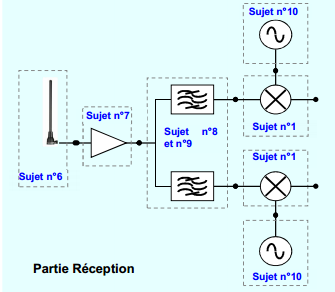
\includegraphics[width=\linewidth]{img/reception}
\end{center}

Comme son nom l'indique, le LNA est un amplificateur faible bruit, il se distingue d'un amplificateur à grand gain par le fait de posséder un gain fixé pour une faible figure de bruit. L'impact du bruit est particulièrement important dans notre cas car nous sommes en charge du premier étage au niveau de la chaîne de d'amplification en réception et nous savons que le bruit global de la chaîne dépend principalement du bruit du premier étage d'amplification.

La conception d'un LNA se distingue d'un amplificateur à gain par son faible bruit : outre le bruit intrinsèque du composant le facteur de bruit (comme le gain) dépend des impédances présentes en sortie et en entrée ainsi que du point de fonctionnement choisi pour le transistor. 

~

On a vu en cours qu'il n'est pas possible d'obtenir le gain le plus élevé et le bruit le plus faible et c'est là toute la difficulté de la conception du LNA: comment trouver le bon compromis gain/bruit et comment concevoir les réseaux d'adaptation d'entrée et de sortie en conséquence ?
Il est également à noter que ce comportement doit être assuré de manière homogène sur toute la bande de fonctionnement de l'amplificateur.

~

Les étapes de conception peuvent être résumées ci-dessous : ce sont celles qui ont été vues en cours d'hyperfréquence:

\begin{enumerate}
\item Définition du cahier des charges
\item Définition du point de fonctionnement
\item Stabilisation et détermination des caractéristiques de gain et de bruit
\item détermination des charges à présenter en entrée et sortie de l'amplificateur afin de
respecter le compromis gain/bruit imposé par le cahier des charges
\item Implémentation de ces charges et validation du résultat
\item Analyse des performances.
\end{enumerate}

\section{Cahier des charges}

Notre principal objectif est d’amplifier à 2.4GHz et 2.5GHz en ayant un facteur de bruit le plus petit possible. À partir du moment où on a un facteur de bruit inférieur à 3dB, on cherche ensuite à avoir le meilleur rapport Gain/Facteur de bruit possible, et tout le reste découle de ce choix.

À partir de là, notre cahier des charges final est le suivant:

\begin{center}
\begin{tabular}{|r|c|l|}
\hline 
grandeur & valeur & unité\\ 
\hline 
Tension d’alimentation & 12 & V \\ 
\hline
$NF_{min}$ & < 3 & dB\\ 
\hline 
NF & $\simeq NF_{min}$ & dB\\ 
\hline 
Gain & $\gg NF$ & dB \\ 
\hline 
$S_{11}/S_{21}/S_{22}$ & $\ll Gain$ & dB \\
\hline
\end{tabular} 
\end{center}

\section{Conception}

\subsection{Choix du transistor}
En regardant les datasheet des NPN, les NF sont entre 1 et 3 pour ceux qui se clament «low noise», tandis que pour les FET c’est entre 0.26 et 0.51, ce qui justifie donc le choix d’un FET.

Les performances des trois transistors sont relativement similaires dans notre cas, donc on décide de prendre l’ATF-54143, qui va nous permettre d’avoir une tension $V_{gs}$ positive, et donc de n’avoir besoin que d’une seule alimentation.

Puisque nous cherchons à minimiser le bruit, on veut éviter la distorsion à tout prix, on se place donc naturellemnt en classe A, qui présente une distorsion théorique nulle.

\subsection{Choix du substrat}

Pour le choix du substrat, on considère essentiellement l’$\varepsilon_r$, et on a le choix entre 10.7 et 2.55. On prendra donc 10.7, le 2.55 étant plutôt réservé aux antennes puisqu’il présente un meilleur rayonnement, et que notre but est également d’éviter les pertes.


\subsection{Circuit de polarisation}
Afin d’appliquer les tensions de polarisation que l’on désire sur notre transistor sans perturber le signal hyperfréquences, nous avons utilisé un circuit similaire à ceux que l’on a vu en TP, en modifiant les caractéristiques du substrat et les largeurs de ligne. 

Après un certain nombre de tests et de \textit{tunes}, nous somme passés à une version entièrement en stubs, dont voici le schéma final:

\begin{center}
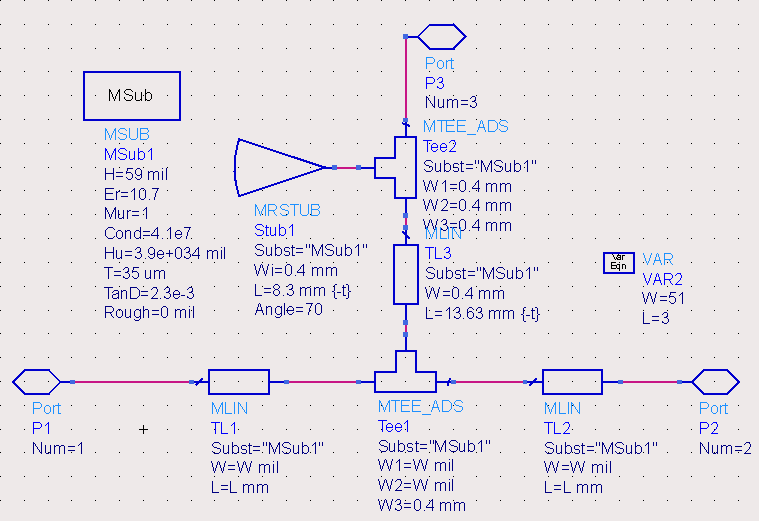
\includegraphics[width=\linewidth]{img/circuit_polar_momentum}
\end{center}

Une fois ce circuit concluant sous Momentum, nous avons utilisé les caractéristiques données par le gerber (ci-dessous) pour l’insérer dans le reste du projet, et baser les simulations futures sur ses caractéristiques.

\begin{center}
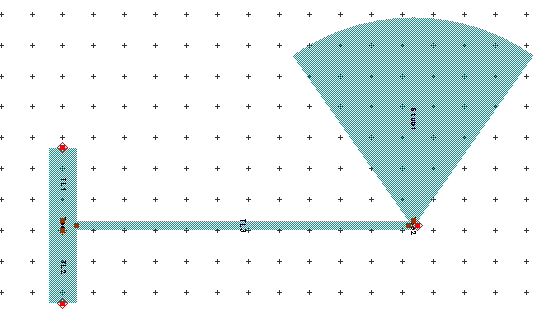
\includegraphics[width=\linewidth]{img/gerber_polar}
\end{center}

\subsection{Polarisation}

Dans un premier temps, nous avions déterminé que les caractéristiques qui nous intéressaient étaient optimales pour un $V_{ds}$ de 3V et un $V_{gs}$ de 0.86V.

Cependant, cela impliquait d’avoir un $I_{ds}$ de 421mA, et on dépassait donc largement les 725mW maximum dissipables par le boitier du transistor.

Puisque la datasheet donne également un $I_{ds}$ maximum de 120mA, nous ne pouvions pas jouer uniquement sur $V_{ds}$ pour faire baisser la puissance consommée, donc nous avons abaissé $V_{gs}$ jusqu’à 0.65V, en gardant $V_{ds}$ à 3V.

Ceci nous donne un $I_{ds}$ de 111mA, ce qui est dans la plage autorisée du transistor, tant en courant qu’en tension et en puissance.

\subsection{Tracé des cercles de gain et de bruit}
En trançant les cercles de gain et de bruit, on se rend compte que le bruit croit très rapidement au début, ce qui est moins vrai pour le gain. On cherche donc à se placer le plus près possible du centre de ces cercles de bruit.

Ceci nous a conduit à choisir un point de fonctionnement où le bruit est de 0.427dB et le gain e 17.7dB:

\begin{center}
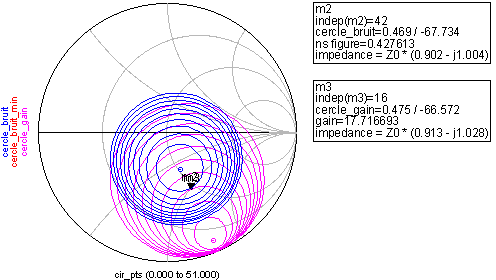
\includegraphics[width=\linewidth]{img/cercles}
\end{center}

On aurait pu naturellement avoir un meilleur bruit \textbf{ou} un meilleur gain, mais tout l’intérêt de la conception d’un LNA réside dans le compromis entre ces deux valeurs. Nous étions partis avec une idée générale d’un bruit inférieur à 3dB pour un gain supérieur à 10, donc en ayant un bruit inférieur à 0.5 et un bruit supérieur à 17, nous pensons qu’en passant à la version réele et donc en perdant un peu de gain et en gagnant un peu de bruit, on restera largement dans ce cahier des charges initial.

Étant donné que le bruit reste notre contrainte prépondérante, nous préférons prendre plus de marge sur le bruit que sur le gain. Ainsi, si on peut garder un NF le plus bas possible, c’est mieux.

\subsection{Circuits d’adaptation}

Ces deux circuits ont été développés en éléments répartis, par la méthode de l'adaptation simple stub, à partir du point choisi sur l’abaque de Smith précédente, et en utilisant l’outil \textit{Smith Chart Utility}

Voici le schéma en «MLIN» final pour l’entrée:

\begin{center}
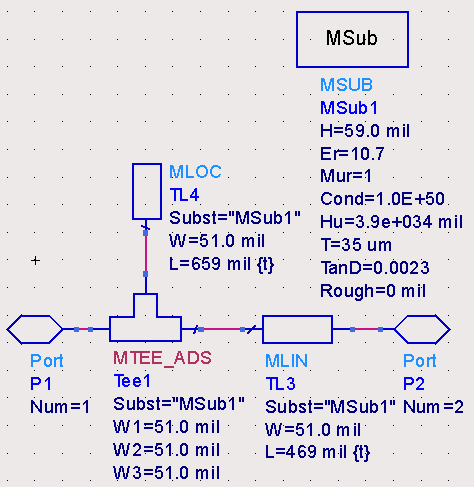
\includegraphics[width=\linewidth]{img/reseau_adapt_entree}
\end{center}

L'impédance à ramener en sortie étant de partie imaginaire pratiquement nulle nous avons décidé de nous passer du stub et de modifier la partie réelle grâce à une transition $50-35 \Omega$.

\newpage

\subsection{Circuit final pour la simulation}

Une fois toutes les différentes parties du circuit assemblées, nous obtenons ceci pour nos simulations et nos derniers \textit{tunes}:

\begin{center}
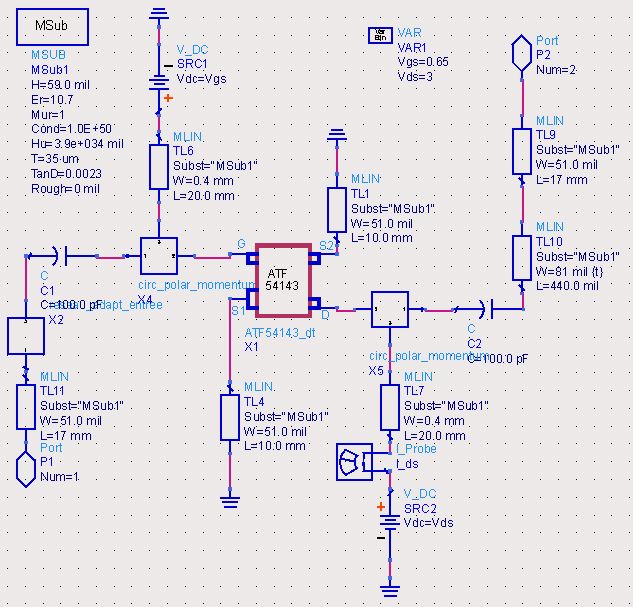
\includegraphics[width=\linewidth]{img/simu_final}
\end{center}

\subsection{Paramètres S finaux en simulation}

\begin{center}
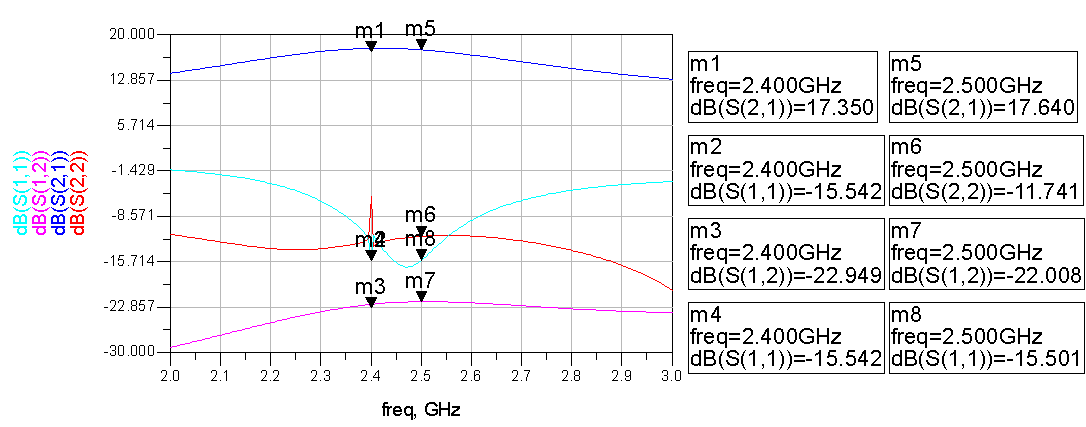
\includegraphics[width=\linewidth]{img/param_S_simu}
\end{center}

On a fait un effort pour avoir les paramètres S à 2.4GHz et 2.5GHz pratiquement égaux, et donc on a perdu un peu en performances, mais avec un gain de 17dB, on est encore très largement dans le cahier des charges initial, et, si tout se passe bien, il parait peu probable de perdre beaucoup plus de 7dB en passant de la simulation à la fabrication.

\subsection{Retour sur le cahier des charges}

\begin{center}
\begin{tabular}{|r|c|c|l|}
\hline 
 & Fixé & Simulé & Unité\\ 
\hline 
Tension d’alimentation & 12 & 12 & V \\
\hline 
$NF_{min}$ & < 3 & 0.315 & dB\\ 
\hline 
NF & $\simeq NF_{min}$ & 0.43 & dB\\ 
\hline 
Gain & > 10 & 17.35 & dB \\ 
\hline 
$S_{11}/S_{21}/S_{22}$ & $\ll Gain$ & <Gain-20 & dB \\
\hline
\end{tabular} 
\end{center}

Pour les étapes de conception, nous semblons donc être largement dans le cahier des charges initial.

\subsection{Circuit final pour la fabrication}

Le circuit précédent était bon pour des simulations, mais lorsqu’il s’agit de fabriquer le circuit, il n’est plus valable, puisqu’il reste certains éléments idéaux (comme les capacités) et que nous avons besoins de lignes d’accès pour connecter physiquement les différents fils sur le circuit imprimé. Nous avons donc du modifier le circuit de simulation pour le circuit suivant:

\begin{center}
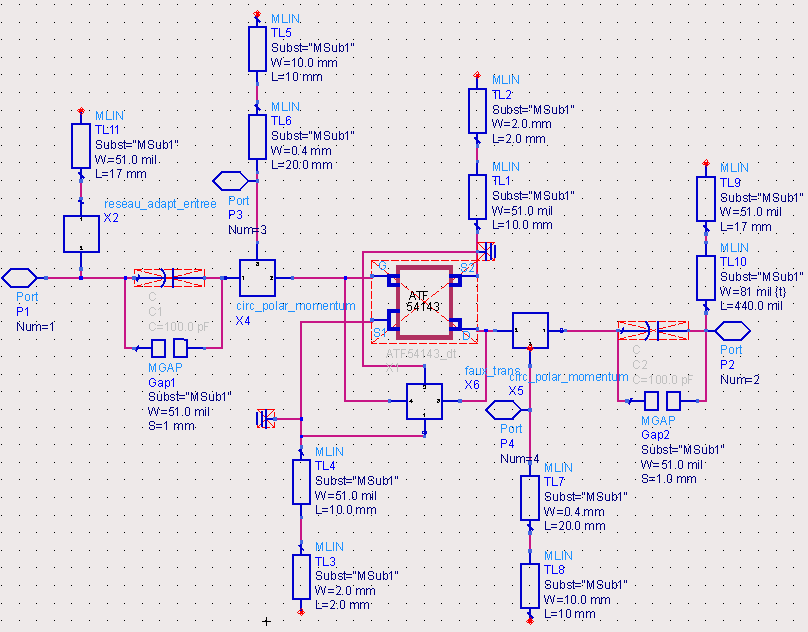
\includegraphics[width=\linewidth]{img/circuit_pour_gerber}
\end{center}

Le «faux\_trans» est une empreinte Momentum que nous avons dessinée à partir de la datasheet de notre transistor, et les «MGAP» sont des espaces de 1mm sur les lignes d’accès, et servent à positionner les capacités réelles.

Les «MLIN» longs supplémentaires servent à déporter les accès, et les «MLIN» plus large à leur extrémité servent à venir souder les fils et les résistances dont nous avons besoin pour créer la tension de polarisation à partir de la tension d’alimentation du circuit.

~

Une fois ce circuit terminé, nous obtenons un fichier gerber que nous avons fait fabriquer:

\begin{center}
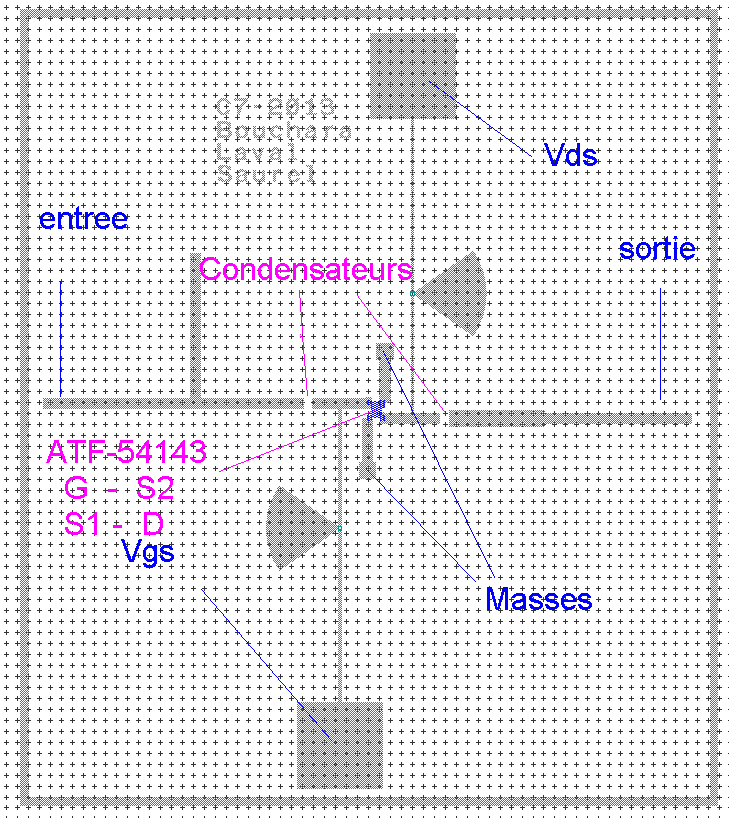
\includegraphics[width=\linewidth]{img/gerber_final}
\end{center}

\section{Fabrication et performances}

\subsection{Premières impressions}

Une fois le transistor et les condensateurs soudés, nous avons remarqué que nous avions oublié les «MGAP» pour le pont de résistances qui sert à la polarisation. Ce problème à été rapidement résolu à l’aide d’un coup de cutter bien placé.

~

Après avoir soudé les différents composants et vérifié les tensions de polarisation, nous avons essayé d’envoyer un signal modulé sur l’entrée, et d’observer la sortie. Comme rien ne marche jamais du premier coup, nous avons cherché à quel endroit nous avions pu perdre une bonne partie de nos performances entre la simulation et la réalité, et nous en avons déduit que les lignes d’accès au masses (pattes S1 et S2 du transistor) étaient beaucoup trop longues. 

Les enlever nous a redonné à la fois de bonnes caractéristiques et un peu d’espoir pour la suite.

\subsection{Paramètres S}
Le premier indicateur de performances que nous avons utilisé est une mesure des paramètre S de notre circuit (ce rendu réalisé sous ADS est obtenu à partir d’un fichier généré par l’analyseur de réseau):

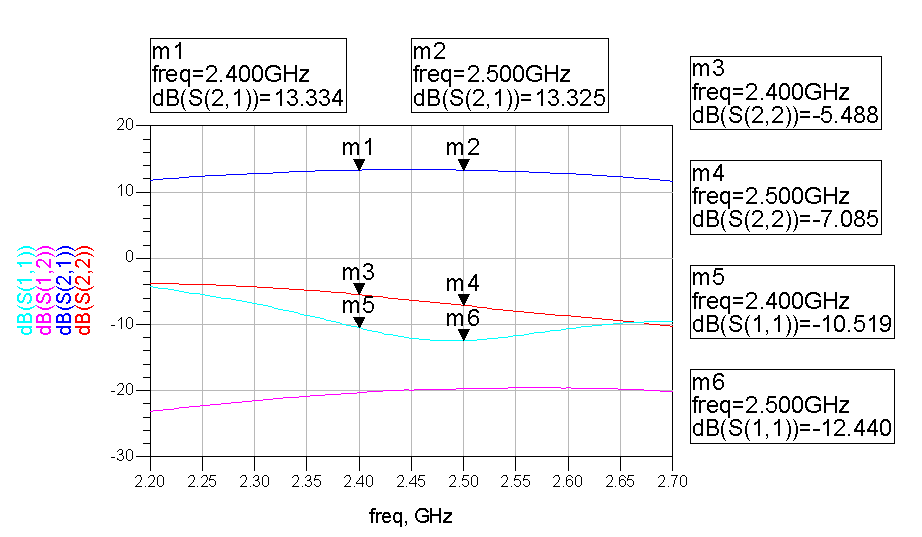
\includegraphics[width=\linewidth]{img/S_reels}

Le gain est descendu entre la simulation et la pratique de 17dB à 13dB, mais on reste sans problèmes dans notre cahier des charges initial.

\subsection{Bruit}

On était à 0.4 en simulation, est on est passé à 0.7, donc c’est resté tout à fait satisfaisant.

\subsection{Linéarité}

En faisant varier la puissance que l’on injecte dans notre LNA, on regarde la puissance en sortie (ici, on n’a que 10.4dB de gain, mais il faut considérer la perte dans les câbles):

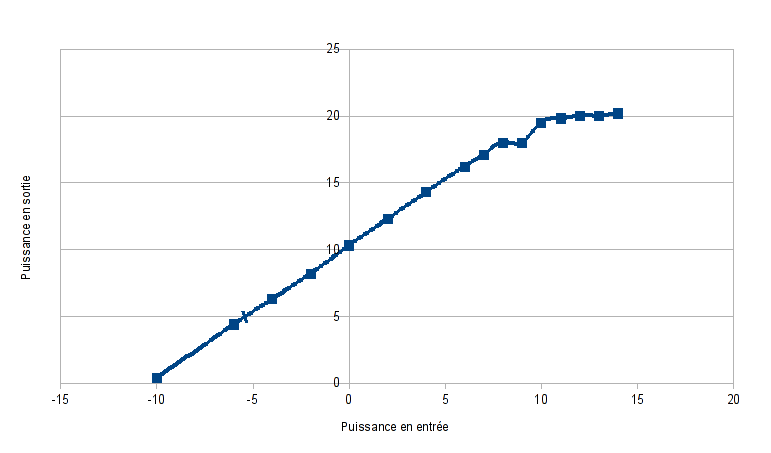
\includegraphics[width=\linewidth]{img/linearite}

Notre montage est donc tout à fait linéaire jusqu’à une puissance en entrée d’au moins 5dBm. Il est peu probable que le signal reçu par l’antenne à l’étage d’avant soit supérieur à cette puissance.

\subsection{Influence des raies d’intermodulation}

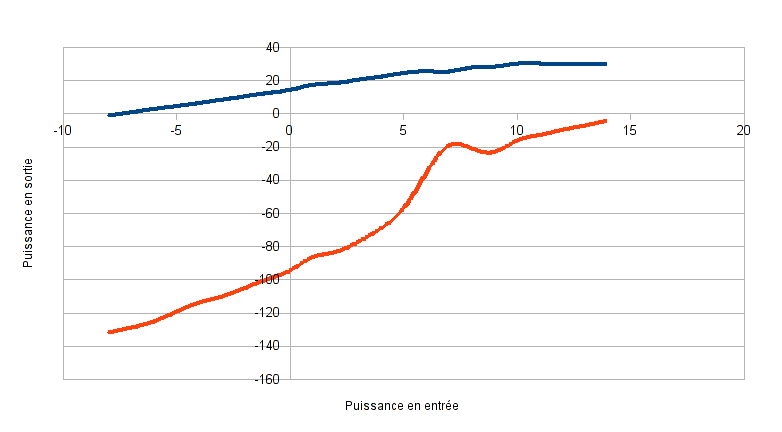
\includegraphics[width=\linewidth]{img/IP3}

La courbe en bleu représente la somme des puissances des raies à 2.4GHz et 2.5GHz, et la rouge représente la somme des puissances des raies d’intermodulation de rang 1.

Le point de compression à 3 dB se situe donc d’après ces courbes largement après les 5dBm de fin de linéarité.

Ces résultats sont pour des mesures autour de 2,45GHz, et pas tout à fait à 2.4GHz et 2.5GHz, puisque nous n’avions pas accès à un mélangeur suffisamment large bande.


\subsection{Retour sur le cahier des charges}

\begin{center}
\begin{tabular}{|r|c|c|c|l|}
\hline 
 & Fixé & Simulé & Mesuré & Unité\\ 
\hline 
Tension d’alimentation & 12 & 12 & 12 & V \\
\hline 
$NF_{min}$ & < 3 & 0.315 & N/A & dB\\ 
\hline 
NF & $\simeq NF_{min}$ & 0.43 & 0.7 & dB\\ 
\hline 
Gain & > 10 & 17.35 & 13 & dB \\ 
\hline 
$S_{11}/S_{21}/S_{22}$ & $\ll Gain$ & < Gain-20 & <Gain-15 & dB \\
\hline
\end{tabular} 
\end{center}

Notre cahier des charges n’était pas particulièrement chargé, donc nous n’avons pas eu beaucoup de mal à le tenir.

La seule contrainte qui nous aura posé problème à travers une perte non négligeable de temps aura été la tenue en puissance du transistor que nous avons choisi, ce qui fait également implicitement partie du cahier des charges.

\section{Conclusion}

Ce projet fut très enrichissant tant au niveau théorique que technique. Ce projet nous a permis de mettre en pratique la théorie apprise en hyperfréquence durant le premier semestre. Nous avons fait face aux difficultés imposées par le projet à savoir que le projet était assez "libre" au niveau du cahier des charges par exemple.

La nécessité d'avoir une démarche d'analyse et synthèse est primordiale pour ne pas se perdre dans le projet et pour voir l'avancement de ce dernier.

Le travail d'équipe, le recherche et l'analyse des résultats nous ont permis de respecter le cahier des charges.

~

Nous tenons à remercier l'ensemble des professeurs pour leur aide et leurs conseils avisés durant le projet, notamment parce qu’ils nous ont laissé une grande liberté à tous les niveaux de conception tout en étant capable de nous aider très rapidement lorsque nous avions un problème.


\end{document}